\chapter{Qualitative Methods, Numerical Methods, and Bifurcations}
Let's think about the by-hand calculus techniques for differentiation and integration for
a minute.  If you were to ask someone for a function then so long as the person gave you
the algebraic form of the function you could always differentiate it.  Always! By hand
derivatives, in some sense, are easy.  We have
differentiation techniques to take care of every algebraic function.  Integration, on the
other hand, is a different beast.  If you are handed some random algebraic function then
you would find that it is very rare that an antiderivative exists.  Of course we have the
ideas of $u$ substitution, integration by parts, trig substitution, partial fractions,
etc. to take care of the most common cases, but most algebraic functions simply don't have
antiderivatives.  What do you do in the cases where an antiderivative doesn't exist?
Well, if you're trying to use the fundamental theorem of calculus to get a definite
integral you can always revert to Riemann sums and use a computer. You could also use the
trapezoidal rule or some other approximation technique, but that is about it;
approximation is the only recourse in most instances.

The same types of troubles arise with differential equations.  We saw in the first chapter that if
we have a first order differential equation then we have a few techniques at our disposal
to get an analytic solution,
but we most certainly can't solve every differential equation.  Take for example the
differential equation $y' = \ln(\sin(\ln(xy)))\sin(x^2)$ \ldots good luck getting an
analytic solution.  The analytic solution to a
differential equation might be the gold standard goal of differential equations, but it
may come as a surprise that analytic solutions are actually rare and special unicorns.
What we build in this chapter is a collection of techniques designed to find qualitative
or approximate solutions to differential equations without actually trying to get analytic
solutions.  We will rely heavily on graphical intuition and at times we will rely on
computers to do the heavy lifting. By the end of this chapter you'll see that we often
times don't even need the analytic solution since our qualitative analysis can tell us a
wealth of information about the differential equation.


\newpage \section{Equilibrium Points and Stability}
\begin{definition}[Equilibrium Point(s)]
    A point $y=p$ is said to be an {\bf equilibrium point} of a differential equation if
    $y'=0$ for all time when $y=p$.  That is to say that when $y=p$ the rate of change of $y$ is zero
    and as such cannot change with time.
\end{definition}

\begin{definition}[Stability]
    An equilibrium point $y=p$ of a differential equation can be classified as either {\bf
    stable}, {\bf unstable}, or {\bf semi-stable}.  
    \begin{itemize}
        \item At a {\bf stable equilibrium}, small deviations from $y=p$ will result in the
            system converging back to $y=p$ over time.
        \item At a {\bf unstable equilibrium}, small deviations from $y=p$ will result in the
            system diverging away from $y=p$ over time.
        \item At a {\bf semi-stable equilibrium}, small deviation in one direction from
            $y=p$ will result in the system converging back to $y=p$ over time, and small
            deviations in the other direction will result in the system diverging away
            from $y=p$ over time.  We can think of a semi-stable equilibrium as being
            stable from one direction and unstable from another.
    \end{itemize}
\end{definition}


A first order autonomous differential equation may have an equilibrium point where the
change simply stops.  In this section we will build the tools necessary to
find and analyze equilibrium points for autonomous first order differential equations.

\begin{problem}
    The equilibrium point of a first order autonomous differential equation $y'(t) = f(y)$ is defined as
    the value of $y$ where $y'=0$.  
    \begin{itemize}
        \item[(a)] Why is this called an equilibrium point?
        \item[(b)] Find the equilibrium for the first order autonomous differential equation
            \[ y' = -0.5y^2 + 8 \]
        \item[(c)] Make a plot with $y'$ on the vertical axis on $y$ on the horizontal axis for
            the previous differential equation.  Use this plot to determine whether the
            equilibrium point is stable or unstable.
        \item[(d)] Use the \texttt{dfield} software to make a slope field for this
            differential equation.  Tie your findings from parts (b) and (c) to what you
            see in the slope field.
        \item[(e)] Now consider the slightly different differential equation $y' = 0.5 y^2
            + 8$.  Make a plot with $y'$ on the vertical axis and $y$ on the horizontal
            axis.  Use this plot to determine whether the equilibrium is stable or
            unstable.  Then use \texttt{dfield} to verify your classifications of the
            equilibria.
    \end{itemize}
\end{problem}
\solution{
    The equilibrium is $y_{eq} = \sqrt{3/0.2} = \sqrt{15}$.  Stable
}


\begin{problem}
    The air resistance on a sky diver is proportional to the \underline{square} of the velocity.
    Newton's 2nd law can be used to get a differential equation for the velocity of the
    sky diver.
    \begin{enumerate}
        \item Write the differential equation for the velocity (take {\it down} to be
        positive).  You might want to start with a free body diagram and consider the
        balance of forces.  \ldots What Would Newton Do? (WWND)
        \item Find the equilibrium (AKA: terminal velocity) in terms of the mass and the
            proportionality constant for air resistance. How many equilibria are there?
            Discuss their stability.
    \end{enumerate}
\end{problem}
\solution{
    \[ mv' = mg - kv^2 \]
    \[v_{eq} = \sqrt{\frac{mg}{k}} \]
    So for every $k$ there is a terminal velocity, but as $k$ gets larger the terminal
    velocity goes down.
}


\begin{problem}
    Create a first order autonomous differential equation that has 2 unstable equilibria
    and 1 stable equilibrium.\\
    Hint\#1: Use the plot of $y'$ vs $y$ to help.\\
    Hint\#2: Write the right-hand side of your DE to in factored form.
\end{problem}
\solution{
$y' = (y-1)(y-2)(y-3)$ will be unstable at $y=1$ and $y=3$ but stable at $y=2$.
}


\begin{problem}
    A trout pond has a carrying capacity of 200 fish.  Suppose that the trout population
    can be modeled according to the logistic equation
    \[ \frac{dP}{dt} = kP\left( 1-\frac{P}{200} \right) \]
    where $k$ is the intrinsic growth rate of the population.  For the sake of simplicity
    in this model let's assume that $k = 0.5$ (for now).  
    \begin{enumerate}
        \item[(a)] Make a plot with $dP/dt$ on the vertical axis and $P$ on
            the horizontal axis.  Use the differential equation to sketch this plot.
%             \begin{center}
%                 \begin{tikzpicture}
%                     \draw[->,thick, black] (0,0) -- (5,0) node[anchor=west]{$P$};
%                     \draw[->,thick, black] (0,-1) -- (0,3)
%                     node[anchor=south]{$\frac{dP}{dt}$};
%                 \end{tikzpicture}
%             \end{center}
        \item[(b)] Mark the intercepts on the horizontal axis in the plot above.  What do
            they represent in the context of this problem?
        \item[(c)] What does it mean about the rate of change of the population if  the
            plot lies above the horizontal axis?  What about below?
        \item[(d)] Use your answer in part (c) to classify the two equilibrium points as
            either stable or unstable.
    \end{enumerate}
\end{problem}
\solution{
    \begin{enumerate}
        \item[(a)] This is a downward facing parabola with roots at 0 and 200.
        \item[(b)] The intercepts are where $P'=0$ so the rate of change is zero.  These
            are the equilibrium points.
        \item[(c)] If the curve is above the horizontal axis then the rate of change is
            positive.  If the curve is below the horizontal axis then the rate of change
            is negative.
        \item[(d)] 0 is unstable and 200 is stable.
    \end{enumerate}
}


\begin{problem}
    Use what you learned in the previous problems to find and classify the equilibria for the
    first order non-linear autonomous differential equation
    \[ y'(t) = (y-1)(y-2)(y-3)^2. \]
\end{problem}
\solution{
1 is stable, 2 is unstable and 3 is semi-stable
}

\newpage

\begin{technique}[Phase Line Analysis]
    It is often very helpful to draw a {\it phase diagram} (sometimes called a phase line)
    to analyze the equilibrium points of an autonomous differential equation.  There are
    four possible cases shown graphically in Figure \ref{fig:phaseline}.  In each of the
    following fill in with the word(s) ``stable'', ``unstable'', ``semi-stable approaching
    from below'', or ``semi-stable approaching from above''.
    \begin{itemize}
        \item In Case \#1 there is a/an \underline{\hspace{1.5in}} equilibrium at $y=2$.
        \item In Case \#2 there is a/an \underline{\hspace{1.5in}} equilibrium at $y=2$.
        \item In Case \#3 there is a/an \underline{\hspace{1.5in}} equilibrium at $y=2$.
        \item In Case \#4 there is a/an \underline{\hspace{1.5in}} equilibrium at $y=2$.
    \end{itemize}
\end{technique}
\solution{
    \begin{itemize}
        \item Case \#1: unstable
        \item Case \#2: semi-stable approaching from below
        \item Case \#3: stable 
        \item Case \#2: semi-stable approaching from above
    \end{itemize}
}

\begin{figure}[h]
    \begin{center}
        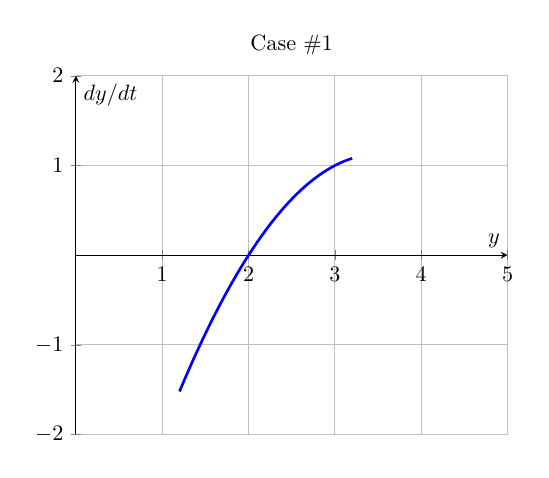
\begin{tikzpicture}[scale=0.8]
            \begin{axis}[axis lines=center, grid, domain=0:5, xlabel={$y$},
                    ylabel={$dy/dt$}, title={Case \#1}, xmin=0, xmax=5, ymin=-2, ymax=2]
                    \addplot[blue, domain=1.2:3.2, very thick, smooth] {-0.5*(x-2)*(x-5)};
            \end{axis}
        \end{tikzpicture}
        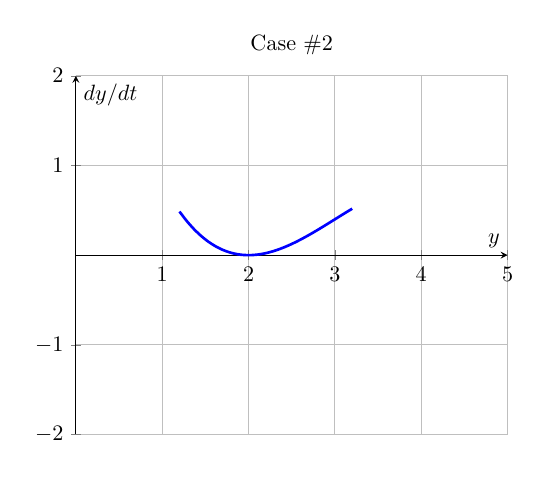
\begin{tikzpicture}[scale=0.8]
            \begin{axis}[axis lines=center, grid, domain=0:5, xlabel={$y$},
                    ylabel={$dy/dt$}, title={Case \#2}, xmin=0, xmax=5, ymin=-2, ymax=2]
                    \addplot[blue, domain=1.2:3.2, very thick, smooth] {-0.2*(x-2)^2*(x-5)};
            \end{axis}
        \end{tikzpicture}
        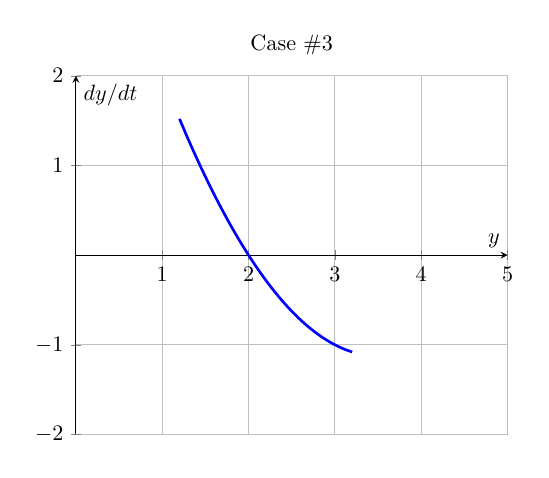
\begin{tikzpicture}[scale=0.8]
            \begin{axis}[axis lines=center, grid, domain=0:5, xlabel={$y$},
                    ylabel={$dy/dt$}, title={Case \#3}, xmin=0, xmax=5, ymin=-2, ymax=2]
                    \addplot[blue, domain=1.2:3.2, very thick, smooth] {0.5*(x-2)*(x-5)};
            \end{axis}
        \end{tikzpicture}
        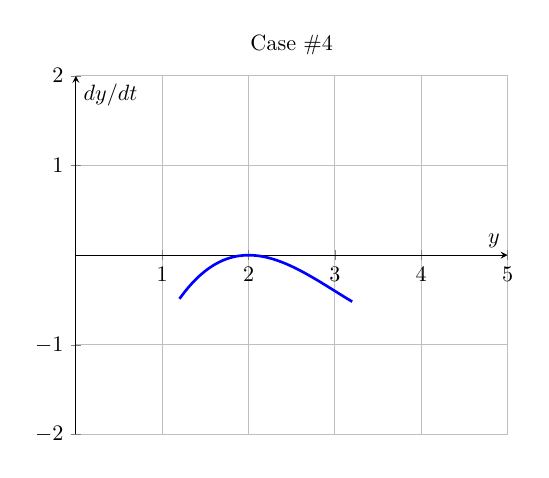
\begin{tikzpicture}[scale=0.8]
            \begin{axis}[axis lines=center, grid, domain=0:5, xlabel={$y$},
                    ylabel={$dy/dt$}, title={Case \#4}, xmin=0, xmax=5, ymin=-2, ymax=2]
                    \addplot[blue, domain=1.2:3.2, very thick, smooth] {0.2*(x-2)^2*(x-5)};
            \end{axis}
        \end{tikzpicture}
    \end{center}
    \caption{Four cases for phase line analysis. In each plot we see a small portion of
        the $\frac{dy}{dt}$ vs $y$ plot for an autonomous first order differential
        equation: $\frac{dy}{dt} = f(y)$.}
    \label{fig:phaseline}
\end{figure}

\newpage


\begin{problem}
    For each of the phase plots in Figure \ref{fig:phase2} sketch a plot on the  $y$ vs
    $t$ plane of the solutions
    to the underlying differential equation. A few helpful markers are given to
    you in the first plot.
\end{problem}

\begin{figure}[h]
    \begin{center}
        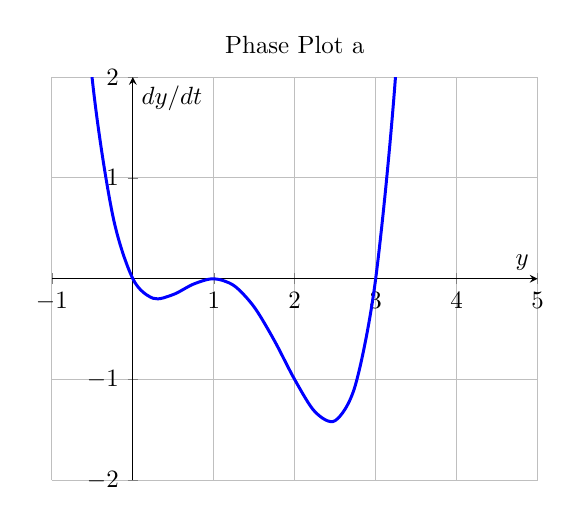
\begin{tikzpicture}[scale=0.9]
            \begin{axis}[axis lines=center, xlabel={$y$}, ylabel={$dy/dt$}, grid, xmin=-1,
                xmax=5, ymin=-2, ymax=2, title={Phase Plot a}]
                \addplot[smooth, very thick, blue, domain=-1:5] {0.5*x*(x-1)^2*(x-3)};
            \end{axis}
        \end{tikzpicture}
        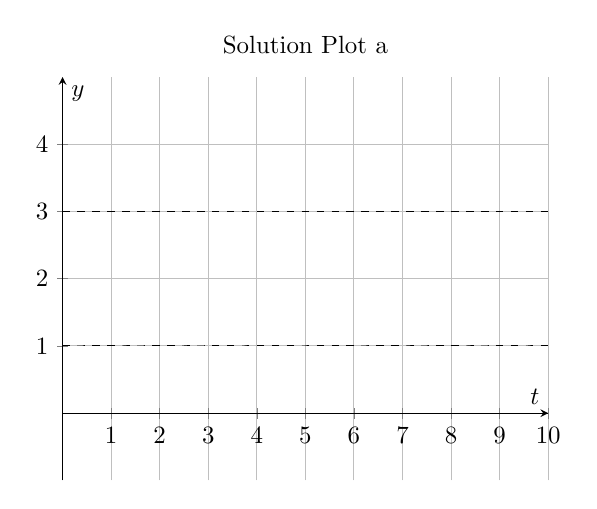
\begin{tikzpicture}[scale=0.9]
            \begin{axis}[axis lines=center, xlabel={$t$}, ylabel={$y$}, grid, xmin=0,
                xmax=10, ymin=-1, ymax=5, title={Solution Plot a}, ytick={1,2,3,4},
            xtick={1,2,3,4,5,6,7,8,9,10}]
                \addplot[dashed, domain=0:10] {0*x+0};
                \addplot[dashed, domain=0:10] {0*x+1};
                \addplot[dashed, domain=0:10] {0*x+3};
            \end{axis}
        \end{tikzpicture}
        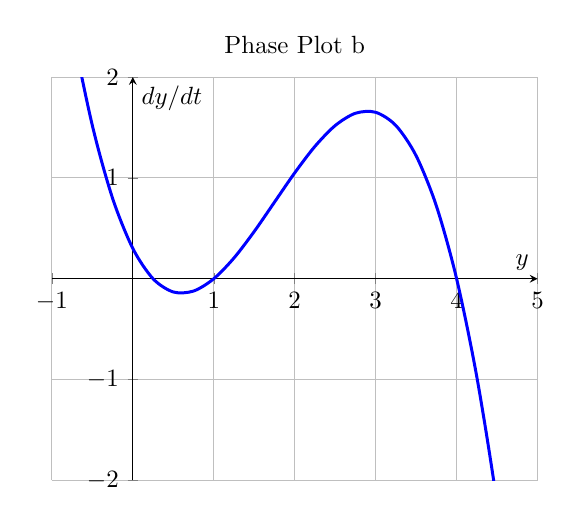
\begin{tikzpicture}[scale=0.9]
            \begin{axis}[axis lines=center, xlabel={$y$}, ylabel={$dy/dt$}, grid, xmin=-1,
                xmax=5, ymin=-2, ymax=2, title={Phase Plot b}]
                \addplot[smooth, very thick, blue, domain=-1:5] {-0.3*(x-0.25)*(x-1)*(x-4)};
            \end{axis}
        \end{tikzpicture}
        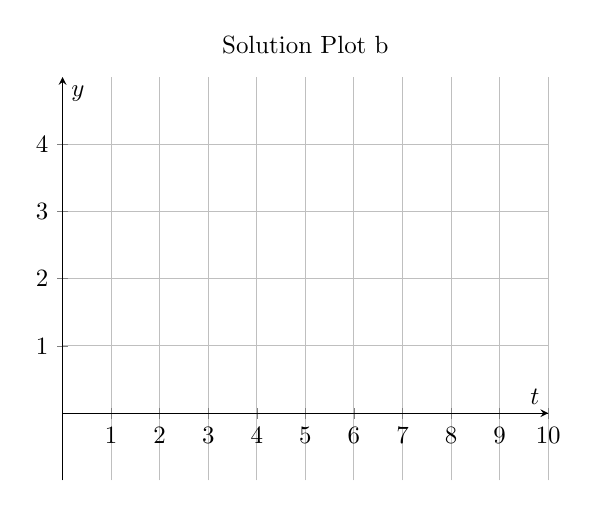
\begin{tikzpicture}[scale=0.9]
            \begin{axis}[axis lines=center, xlabel={$t$}, ylabel={$y$}, grid, xmin=0,
                xmax=10, ymin=-1, ymax=5, title={Solution Plot b}, ytick={1,2,3,4},
            xtick={1,2,3,4,5,6,7,8,9,10}]
                \addplot[smooth, domain=0:10] {0*x+0};
            \end{axis}
        \end{tikzpicture}
    \end{center}
    \caption{Phase plots and solution plots.  On the left are the phase plots and on the
    right are coordinate axes to sketch the solution plots.}
    \label{fig:phase2}
\end{figure}


\begin{example}
    Consider the differential equation $y' = y e^{-y^2}(y-3)$.  Find and classify the
    equilibrium points. \\ {\bf Solution:} \\
    To find the equilibrium points we set $y'$ equal to zero and solve the resulting
    algebraic equation.  Hence we need to solve
    \[ 0 = y e^{-y^2} (y-3) \]
    which yields $y_{eq} = 0$ and $y_{eq} = 3$ (noting that the exponential is never zero).  
    Now we can observe a phase diagram by plotting $y'$ vs $y$ and use this to determine
    stability.
    \begin{center}
        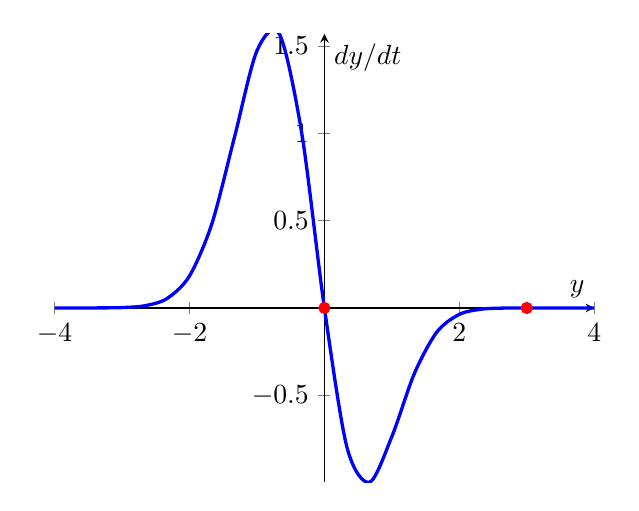
\begin{tikzpicture}
            \begin{axis}[axis lines=center, xlabel={$y$}, ylabel={$dy/dt$}, domain=-4:4]
                \addplot[smooth, blue, very thick] {x*exp(-x^2)*(x-3)};
                \draw[fill=red, color=red] (axis cs:0,0) circle(0.07cm);
                \draw[fill=red, color=red] (axis cs:3,0) circle(0.07cm);
            \end{axis}
        \end{tikzpicture}
    \end{center}
    In the plot above it is clear that to the left of $y=0$ we have $dy/dt > 0$ so the
    solution is increasing (moving to the right).  To the right of $y=0$ we have $dy/dt <
    0$ so the solution is decreasing (moving to the left).  Therefore we conclude that
    $y=0$ is a stable equilibrium point.  At $y=3$, on the other hand, it is hard to tell
    what is happening to the right.  If we put any $y$ value larger than 3 into the
    right-hand side of the differential equation we will get a positive number so even
    though we can't see it in the graph we know that to the right of $y=3$ the solution is
    increasing.  To the left the solution is clearly decreasing.  Hence we conclude that
    $y=3$ is an unstable equilibrium point.
\end{example}


\begin{example}
    Devise a differential equation that has 1 stable equilibrium, 1 unstable equilibrium,
    and 1 semi-stable equilibrium. \\ {\bf Solution:} \\
    We want a differential equation that, when graphed on the $y'$ vs $y$ plane, looks
    something like one of the plot below.  We're going to just arbitrarily choose the equilibrium
    points to be $y=-2, 1,$ and $3$.
    \begin{center}
        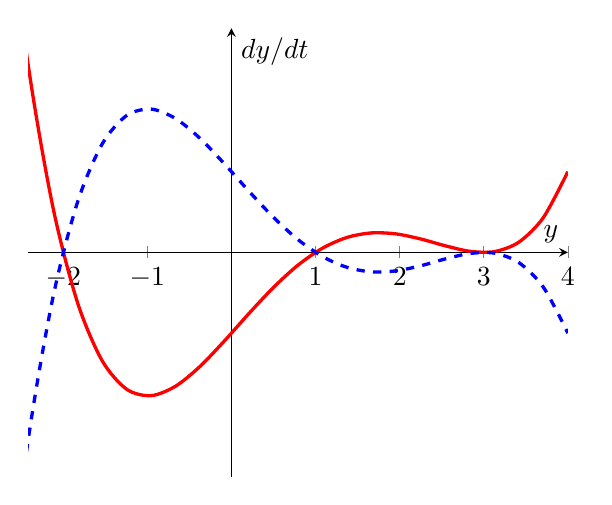
\begin{tikzpicture}
            \begin{axis}[axis lines=center, xlabel={$y$}, ylabel={$dy/dt$}, domain=-3:4,
                ymin=-5, ymax=5, ytick=\empty]
                \addplot[smooth, red, very thick] {0.1*(x+2)*(x-1)*(x-3)^2};
                \addplot[smooth, blue, dashed, very thick] {-0.1*(x+2)*(x-1)*(x-3)^2};
            \end{axis}
        \end{tikzpicture}
    \end{center}
    In both cases we can see that the point $y=3$ is semi-stable.  In on the red solid
    curve we see that $y=-2$ is stable and $y=1$ is unstable.  On the blue dashed curve we
    see that $y=-2$ is unstable and $y=1$ is stable.  If we assume that these curves are
    polynomial functions of $y$ and we know the roots and end behavior then we can write the factored form
    of the functions that generate them.  Indeed, the red curve is generated by the
    function $f(y) = (y+2)(y-1)(y-3)^2$ and the blue dashed curve is generated by the
    function $g(y) = - f(y)$.  Therefore the differential equations are 
    \[ y' = (y+2)(y-1)(y-3)^2 \text{ (red) } \] 
    and
    \[ y' = -(y+2)(y-1)(y-3)^2 \text{ (blue) } \] 
\end{example}

\begin{problem}
    Draw a sketch of all of the solutions to both of the differential equations generated in the
    previous example.  For this problem the vertical axis should be $y$ and the horizontal
    axis should be $t$.
\end{problem}


\newpage


\newpage\section{Numerical Methods}

In this section we will build two numerical solvers that allow you to use a computer to
approximate solutions to the differential equation 
\begin{flalign}
    y' = f(t,y) \label{eqn:ode}
\end{flalign}
for a given initial condition.  In the problems that follow you will be creating several
\texttt{MATLAB} files that you will use throughout the course, so please save them in a
meaningful place and share them with your group mates. Numerical solutions are used when
all else fails.  If you have an analytic solution to your differential equation then there
is no need to make a numerical solution since every numerical solution is only a means of
approximating solutions -- why approximate if you have the exact answer? That being said,
analytic solutions to differential equations are rare so we'll have to approximate more
times than not.

There are MANY approximation techniques for differential equations.  Some are tailored to
specific physics or engineering problems, some are tailored to specific types of initial
or boundary conditions, and others are designed to work on a wide variety of problems.  The two
techniques that we build here are both general purpose and relatively easy to program in
any programming language.  The fact that they are general purpose, however, means that you
can get better performance out of other methods on problems of specific types. To learn
more I encourage you to take a course on numerical analysis.

\subsection{Euler's Method}\label{sec:Euler}
Euler's method is the simplest numerical method for solving the first-order differential equation
$y'=f(t,y)$, and hence it is the best place to start!  You should be familiar with Euler's
method from pre-requisite courses, but this time we are not going to be using Excel (since
we usually need something FAR more powerful!).  

Euler's method is simple: approximate the derivative in the most naive possible way.  That
is, use the definition of the derivative from calculus,
\[ f'(x) = \lim_{h \to 0} \frac{f(x+h) - f(x)}{h}, \]
and just drop the limit.  Therefore we can approximate $y'(t)$ as
\[ \frac{dy}{dt} \approx \frac{y_{new} - y_{old}}{\Delta t}. \]
Then rewrite the differential equation $y' = f(t,y)$ as
\[ \frac{y_{new} - y_{old}}{\Delta t} \approx f(t_{old},y_{old}). \]
After some rearrangement and relabeling we get the difference equation
\[ y_{n+1} = y_n + \Delta t f(t_n,y_n). \]

\begin{technique}[Euler's Method]
    To approximate $y' = f(t,y)$ first choose $\Delta t$ and then implement the difference
    equation
    \[ y_{n+1} = y_n + \Delta t f(t_n,y_n) \]
    using appropriate computer software. 
\end{technique}
Remember that the only reasonable choice for
$\Delta t$ is to make it {\it very small}.  The trade off to choosing $\Delta t$ small
is that it will take more computer memory to approximate the problem.

A way to think about Euler's method is that at a given point, the slope is approximated by
the value of the right-hand side of the differential equation and then we step forward
$\Delta t$
units in time following that slope.  Figure \ref{fig:Euler} shows a depiction of the idea.
Notice in the figure that in regions of high curvature Euler's method will overshoot the
exact solution to the differential equation.  However, taking $h \to 0$ theoretically
gives the exact solution at the tradeoff of needing infinite computational resources.

\begin{figure}[ht!]
    \begin{center}
        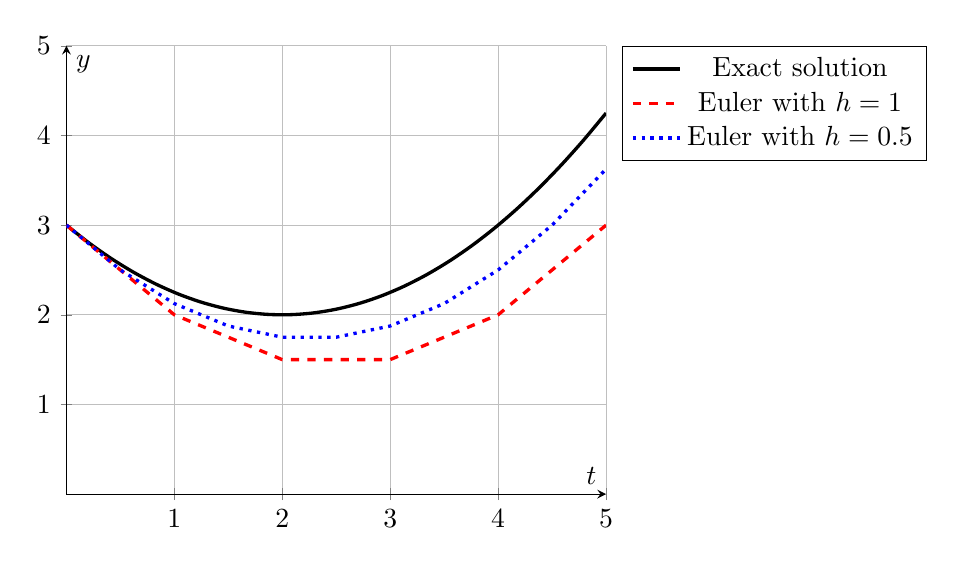
\begin{tikzpicture}
            \begin{axis}[axis lines=center, grid, xmin=0, xmax=5, ymin=0, ymax=5,
                domain=0:5, xlabel={$t$}, ylabel={$y$}, legend pos=outer north east]
                \addplot[very thick, smooth, black] {0.25*(x-2)^2+2};
                \addlegendentry{Exact solution};
                \addplot[red, dashed, very thick]
                coordinates{(0,3)(1,2)(2,1.5)(3,1.5)(4,2)(5,3)};
                \addlegendentry{Euler with $h=1$};
                \addplot[blue, dotted, very thick]
                coordinates{(0,3)(0.5,2.5)(1,2.125)(1.5,1.875)(2,1.75)(2.5,1.75)(3,1.875)(3.5,2.125)(4,2.5)(4.5,3)(5,3.625)};
                \addlegendentry{Euler with $h=0.5$};
            \end{axis}
        \end{tikzpicture}
    \end{center}
    \caption{A depiction of Euler's method with step size $h=1$ (red) and $h=0.5$ (blue).}
    \label{fig:Euler}
\end{figure}


In Figure
\ref{fig:Euler_graphical} we see a graphical depiction of how Euler's method works on the
differential equation $y' = y$ with $\Delta t = 1$ and $y(0) = 1$.  The exact solution
at $t=1$ is $y(1) = e^1 \approx 2.718$ and is shown in red in the figure. 

\begin{figure}[ht!]
    \begin{center}
        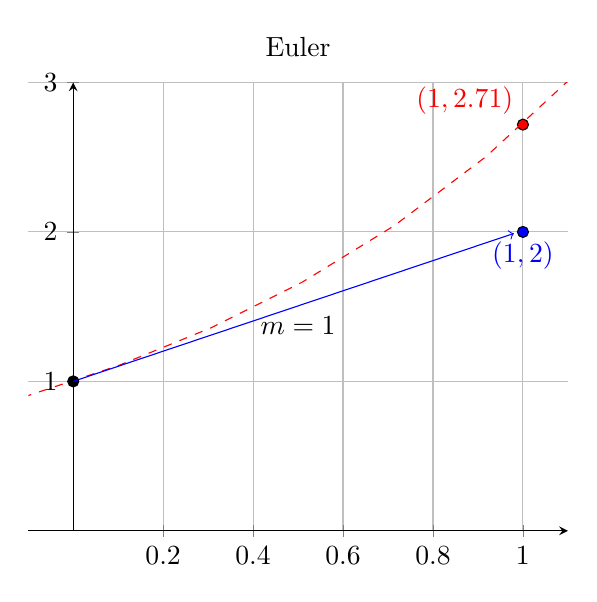
\begin{tikzpicture}
            \begin{axis}[axis lines=center, grid, xmin=-0.1, xmax=1.1, ymin=0, ymax=3,
                title={Euler}]
                \draw[fill=red] (axis cs:1,2.7182) circle(0.07cm); 
                \addplot[dashed, red, samples=50] {1*exp(x)};
                \draw[fill=black] (axis cs:0,1) circle(0.07cm); 
                \draw[blue, ->] (axis cs:0,1) -- (axis cs:0.98,1.99);
                \draw[fill=blue] (axis cs:1,2) circle(0.07cm);
                \draw (axis cs:0.5,1.5) node[anchor=north]{$m=1$};
                \draw[color=blue] (axis cs:1,2) node[anchor=north]{$(1,2)$};
                \draw[color=red] (axis cs:1,2.7182) node[anchor=south east]{$(1,2.71)$};
            \end{axis}
        \end{tikzpicture}
%         \begin{tikzpicture}
%             \begin{axis}[axis lines=center, grid, xmin=-0.1, xmax=1.1, ymin=0, ymax=3,
%                 title={Midpoint}]
%                 \draw[fill=red] (axis cs:1,2.7182) circle(0.07cm); 
%                 \addplot[dashed, red, samples=50] {1*exp(x)};
%                 \draw[fill=black] (axis cs:0,1) circle(0.07cm); 
%                 \draw[fill=blue] (axis cs:0.5,1.5) circle(0.07cm);
%                 \draw[color=blue, dashed] (axis cs:0.4,1.35) -- (axis cs:0.6,1.65);
%                 \draw (axis cs:0.45,1.5) node[anchor=north west]{$m=1.5$};
%                 \draw[color=green!30!black, ->] (axis cs:0,1) -- (axis cs:0.98,2.49);
%                 \draw[fill=green!30!black] (axis cs:1,2.5) circle(0.07cm);
%                 \draw[color=green!30!black] (axis cs:1,2.5) node[anchor=north]{$(1,2.5)$};
%                 \draw[color=red] (axis cs:1,2.7182) node[anchor=south east]{$(1,2.71)$};
%             \end{axis}
%         \end{tikzpicture}
    \end{center}
    \caption{Graphical depiction of Euler's method.  Here we use the simple differential equation
$y'=y$ with $y(0) = 0.5$ and $\Delta t = 1$.  The exact solution is shown in red.}
    \label{fig:Euler_graphical}
\end{figure}



\begin{problem}
    In Excel the process of building an Euler solver is relatively simple.  In \texttt{MATLAB}
it takes a bit more work the very first time, but trust me, the work will pay off in the
long run!
\begin{enumerate}
    \item[(a)] Open \texttt{MATLAB} and create a new \underline{function}.  
    \item[(b)] Change the first line of the function so that it reads \\
        \mcode{function [t,y] = MyEuler(f,tmin,tmax,numpoints,IC)}
    \item[(c)] Explain what each line of code does using comments. Some of the lines of
        code are likely new to you so I suggest you either use the help command or you do
        some basic experimentation.
\begin{lstlisting}
function [t,y] = MyEuler(f,tmin,tmax,numpoints,IC)
t=linspace(tmin,tmax,numpoints);  % what does this line do?
dt=t(2)-t(1); % what does this line do?
y=zeros(size(t)); % what does this line do?
y(1) = IC; % what does this line do?
for n=1:length(t)-1 % what does this line do?
    y(n+1) = ... some code for Euler's method ...
end
\end{lstlisting}
    \item[(d)] Save this code in the working directory for this project.  You also need to
        get \texttt{MATLAB} to look in that working directory.  The simplest way to do
        that is to press F5 while you're in the \mcode{MyEuler} function (and then ignore all of
        the errors that occur).  

        The code you just created works for ALL of the times that you ever need Euler's
        method.  We now just need to create a short script which calls this code and uses
        it.
    \item[(e)] Finally, let's try out your MyEuler code (and at this point you should see why
        you really shouldn't be using Excel for numerical differential equation solvers).
        I'm assuming that you have \texttt{MATLAB} working in the correct directory
        (you'll get errors otherwise!!).  

        We want to get an approximate solution to the differential equation
        \[ y' = -y \cdot \left( 1-\frac{y}{5} \right) + 0.1 t \quad \text{where} \quad
            y(0)=2 \]
            Open a new \underline{script} in \texttt{MATLAB} and complete the following code to get your
        plot.
\begin{lstlisting}
clear; clc; clf;
f = @(t,y) -y*(1-y/5)+0.1*t;
[t,y] = MyEuler(f, ..., ..., ..., ...)
plot(t,y)
grid on
xlabel(...)
ylabel(...)
title(...)
\end{lstlisting}
    \item[(f)] Run your code for several different initial conditions and overlay the plots to
        explore the dynamics of the differential equation. Be sure to properly label your
        plot. It is probably best to do this step within a loop in MATLAB.  To get a
        legend to appear for each new plot you can use the following:
\begin{lstlisting}
clear; clc; clf;
f = @(t,y) -y*(1-y/5)+0.1*t;
LegendItems = { }; % initialize the storage for the legend entries
counter=1; % set up a dummy counter
for IC= ... : ... : ...
  [t,y] = MyEuler(f, ..., ..., ..., ...)
  plot(t,y), hold on
  LegendItems{counter} = ['IC = ' , num2str(IC)]; % what does this line do?
  counter = counter+1; % what does this line do?
end
legend(LegendItems)
\end{lstlisting}
\end{enumerate}
\end{problem}

\begin{problem}
    Run an Euler solver on the differential equation
        \[ y' = -y\left( 1-\frac{y}{5} \right)^2 + \sin(t) \]
        for several different initial conditions. Save your plot in an appropriate place
        with appropriate labels and title.
\end{problem}

\subsection{Runge-Kutta Method}
Euler's method is one of MANY different numerical differential equation solvers.  The
second one that we are going to study in this section is called the Runge-Kutta 4 solver.
The idea is basically the same as with Euler's method: approximate the derivative and
rewrite the differential equation as a difference equation.  The
difference here is that the algorithm is a bit more complex.  \dots Here it is:\\

\begin{technique}[Runge Kutta Method]
First define the dummy variables $k_1, k_2, k_3,$ and $k_4$ as
\begin{flalign*}
    k_1 &= f(t_n,y_n) \\
    k_2 &= f(t_n+\frac{\Delta t}{2} , y_n + \frac{\Delta t}{2} k_1) \\
    k_3 &= f(t_n+\frac{\Delta t}{2} , y_n + \frac{\Delta t}{2} k_2) \\
    k_4 &= f(t_n+\Delta t , y_n + \Delta t k_3).
\end{flalign*}
Then we build the difference equation as a weighted sum of the $k_j's$:
\begin{flalign*}
    y_{n+1} &= y_n + \frac{\Delta t}{6} \left( k_1 + 2 k_2 + 2k_3 + k_4 \right).
\end{flalign*}
% See Figure \ref{fig:RK_figure} to show the technique graphically.
\end{technique}

Before we write code to implement the RK4 method we will examine it graphically just as we
did with Euler's method in Figure \ref{fig:Euler_graphical}.  For
simplicity we will examine the differential equation $y' = y$ with initial condition $y(0)
=1$ and $\Delta t = 1$.  In Figure \ref{fig:RK4_graphical} the red dashed line is the
exact solution $y(t) = e^t$.  In this example, $k_1 = 1$, $k_2 = 1.5$, $k_3 = 1.75$, and
$k_4 = 2.75$.  Hence the final slope propagating forward with $\Delta t = 1$ is 
\[ \frac{1}{6} \left(  1 + 2(1.5) + 2(1.75) + 2.75 \right) = 1.708. \]
Propagating this forward from the point $(0,1)$ gives the new point $(1,2.708)$.  Knowing
that $e \approx2.718$ we see a very high level of accuracy even with a really large time
step!

\begin{center}
    \begin{tabular}{|l|}
        \hline
        Runge-Kutta 4 Method Explanation \\ \hline \hline
        1. $k_1$ is the slope evaluated at time $t_n$ \\ 
        Project this slope half a step forward from time $t_n$ to the point $y_1$ \\ \hline
        2. $k_2$ is the slope evaluated at $y_1$ \\ 
        Project the slope $k_2$ half a step forward from time $t_n$ to the point $y_2$
        \\ \hline
        3. $k_3$ is the slope evaluated at the point $y_2$ \\
        Project the slope $k_3$ a full step foward from time $t_n$ to the point $y_3$ \\
        \hline
        4. $k_4$ is the slope evaluated at the point $y_3$ \\ \hline
        5. Project forward with slope $\frac{1}{6}(k_1 + 2k_2 + 2k_3 + k_4)$ from time
        $t_n$ \\ \hline
    \end{tabular}
\end{center}

\begin{figure}[ht!]
    \begin{center}
        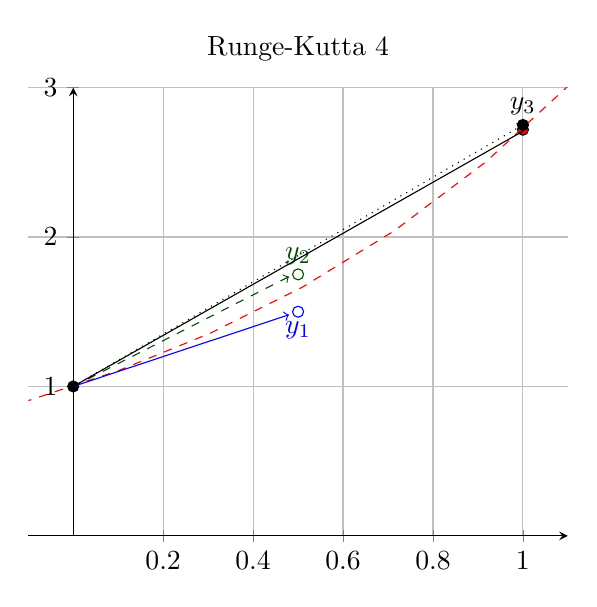
\begin{tikzpicture}
            \begin{axis}[axis lines=center, grid, xmin=-0.1, xmax=1.1, ymin=0, ymax=3,
                title={Runge-Kutta 4}]
                \draw[fill=red] (axis cs:1,2.7182) circle(0.07cm); 
                \addplot[dashed, red, samples=50] {1*exp(x)};
                \draw[fill=black] (axis cs:0,1) circle(0.07cm); 
                \draw[blue,->] (axis cs:0,1) -- (axis cs:0.48,1.48);
                \draw[blue] (axis cs:0.5,1.5) circle(0.07cm) node[anchor=north]{$y_1$};
%                 \draw (axis cs:0.05,1.1) node[anchor=north west]{$k_1 = 1$};
                \draw[color=green!30!black, dashed, ->] (axis cs:0,1) -- (axis
                cs:0.48,1.735);
                \draw[color=green!30!black] (axis cs:0.5,1.75) circle(0.07cm);
                \draw[color=green!30!black] (axis cs:0.5,1.75) node[anchor=south]{$y_2$};
                \draw[color=black, dotted, ->] (axis cs:0,1) -- (axis cs:1,2.75);
                \draw[fill=black] (axis cs:1,2.75) circle(0.07cm);
                \draw (axis cs:1,2.75) node[anchor=south]{$y_3$};
                \draw (axis cs:0,1) -- (axis cs:1,2.708);
            \end{axis}
        \end{tikzpicture}
    \end{center}
    \caption{Graphical depiction of the RK4 method.  The red dashed curve gives the exact
    solution to the differential equation $y' = y$ with initial condition $y(0) = 1$. The
solid black line gives the final projection.}
    \label{fig:RK4_graphical}
\end{figure}

% \begin{problem}
%     Explain the Runge Kutta method graphically.
% \end{problem}
% 
% \begin{figure}[ht!]
%     \begin{center}
%         \begin{tikzpicture}
%             \begin{axis}[axis lines=center, xmin=0, xmax=3.5, ymin=0,
%                     ymax=6,xtick=\empty,ytick=\empty,
%                 legend pos=north east]
%                 \draw[black, dashed] (axis cs:1,0) node[anchor=north]{$t_0$} -- (axis cs:1,6);
%                 \draw[black, dashed] (axis cs:3,0) node[anchor=north]{$t_1$} -- (axis cs:3,6);
%                 \addplot[very thick, domain=1:3, black] {(x-1)^2+1};
%                 \addlegendentry{$y(t)$};
%                 \draw[dashed, red, very thick] (axis cs:1,1) -- (axis cs:3,5);
%                 \draw[dashed, blue, very thick] (axis cs:1,1) -- (axis cs:2,1);
%                 \draw[black, fill=black, very thick] (axis cs:1,1)  circle(0.075cm);
%                 \draw[red, very thick] (axis cs:3,5)  circle(0.075cm);
%                 \draw[green!50!black, very thick] (axis cs:2,1)  circle(0.075cm);
%                 \draw[green!50!black] (axis cs:1.8,0.6) -- (axis cs:2.2,1.4);
%                 \draw[green!50!black, very thick, dashed] (axis cs:1,1) -- (axis cs:2,3);
%                 \addlegendentry{$2$};
% %                 \draw[dashed, red, very thick] (axis cs:1,1) circle(0.075cm) -- (axis cs:3,5)
% %                 circle(0.075cm);
%             \end{axis}
%         \end{tikzpicture}
%     \end{center}
%     \caption{The Runge Kutta method.}
%     \label{fig:RK_figure}
% \end{figure}
% 

\newpage

\begin{problem}
    \begin{enumerate}
        \item[(a)] Create a new function called \texttt{MyRungeKutta} in \texttt{MATLAB} and copy
            all of your code from your \texttt{MyEuler} function.
        \item[(b)] Modify the loop from the Euler code so that you perform the Runge-Kutta
            iteration.  The skeleton code should get you going:
\begin{lstlisting}
...
for n=1:length(t)-1
k1 = ...
k2 = ...
k3 = ...
k4 = ...
y(n+1) = y(n) + ...
end
\end{lstlisting}
        \item[(c)] Run your Runge-Kutta code the same way that you did your Euler code.  Test it
            out on the same two problems as before, and be sure that you get the same
            qualitative solutions.
    \end{enumerate}
\end{problem}


% \subsection{Comparison of Euler and Runge-Kutta}
What we're about to do next should seem a bit silly.  We're going to compare our two
numerical solvers to a differential equation where we HAVE the analytic solution.  You may
be asking yourself ``that seems silly, if you have the analytic solution then why on earth
would you need or want the numerical solution?''  Well, we're going to do it here to prove
a point.  

\begin{problem}
The differential equation in question is: $y' = -5y$.  Solve this equation now by hand (it
should only take a second or two).
\begin{enumerate}
    \item[(a)] Write \texttt{MATLAB} code that solves this differential equation with Euler's
        method and with the Runge-Kutta method for several initial conditions.  Put the
        solutions on top of each other in one subplot.
    \item[(b)] In a second subplot, plot the errors between Euler and the exact solution as
        well as Runge-Kutta and the exact solution.  It would be best to use a
        logarithmically scaled $y$-axis (use \texttt{semilogy} instead of \texttt{plot}).
        Put the results together with several different initial conditions on the same
        plots.
    \item[(c)] What conclusions can you make about the two numerical methods that we have just
        built?  Is one better than the other?  When do they have the largest amount of
        error in general (for any problem)?
\end{enumerate}
\end{problem}

The ideas behind solving ordinary differnetial equations numerically are covered
extensively in a numerical analysis course.  If you're interested I highly recommend that
you take this course.




\newpage\section{Bifurcations}
In this section we will explore the behavior of the equilirium solutions in a differential
equation to changes in a parameter.  In some instances the change in a parameter might
cause the behavior of equilibrium points to change from stable to unstable (or possibly
semi-stable).  It is also possible to {\it spawn} new equilibrium points by changing the
values of parameters. 

It is often the case in real models that parameters are not known with 100\% certainty.
Sometimes the parameters come from scientific measurements, sometimes they are estimated
from data, and sometimes they are just a guess.  If you are in any of these cases with a
first order autonomous differential equation model then you should do a bifurcation
analysis to see how the equilibrium solutions change due to the natural variability in the
parameters.  

\begin{problem}[Fish.net]
    A mathematician at a fish hatchery has been using the differential equation 
    \[ \frac{dP}{dt} = 0.5P\left( 1- \frac{P}{200} \right) \]
    as a model for predicting the number of fish that a hatchery can expect to find in
    their pond.  

    \begin{enumerate}
        \item[(a)] What are the equilibrium points of the mathematician's model.  Discuss their
            stability.  Show the equilibrium points with a plot of $\frac{dP}{dt}$ vs.
            $P$, a phase line, and a slope field.  
        \item[(b)] What does the differential equation predict about the future of the
            fish population for several different initial populations? 
        \item[(c)] Recently the hatchery was bought out by \texttt{fish.net} and the new
            owners are planning to allow the public to catch fish at the hatchery (for a
            fee of course).  This means that the previous differential equation used to
            predict future fish populations needs to modified to reflect this new plan.
            For the sake of simplicity, assume that the managers from \texttt{fish.net}
            are going to allow a constant annual harvest rate $k$.  Which of the four
            modified differential equations makes the most sense to you and why?
            \begin{flalign*}
                & (i) \qquad \frac{dP}{dt} = 0.5 P\left( 1-\frac{P}{200} \right) - k \\
                & (ii) \qquad \frac{dP}{dt} = 0.5 P\left( 1-\frac{P}{200} \right) - kP \\
                & (iii) \qquad \frac{dP}{dt} = 0.5 P\left( 1-\frac{P}{200} \right) - kt\\
                & (iv) \qquad \frac{dP}{dt} = 0.5 P\left( 1-\frac{P-k}{200} \right) 
            \end{flalign*}
        \item[(d)] Using the modified differential equation agreed upon from the previous
            problem, discuss the implications that various choices of $k$ will have on
            future fish populations.  In particular, are there choices of $k$ that change
            the nature or number of the equilibrium points?  Defend your work graphically
            and analytically.
%         \item Find the equilibrium points in terms of the model parameters.
%         \item When are there 2, 1, or 0 equilibrium points?
%         \item Draw a plot with the parameter $h$ on the horizontal axis and the value of
%             the equilibrium point(s) on the vertical axis. Use $M = 1$ and $k = 1$ for
%             simplicity.
    \end{enumerate}
\end{problem}
% \solution{
%     \[ \frac{dP}{dt} = kP(M-P) \]
%     has equilibria $P=0$ and $P=M$ (unstable and stable resp.)
% 
%     For a harvesting model:
%     \[ \frac{dP}{dt} = kP(m-P)-h \]
%     Therefore,
%     \[ 0 = kP(M-P)-h \implies -kP^2 _ kMP - h = 0 \implies P = \frac{-kM \pm \sqrt{k^2M^2
%     - 4kh}}{-2k} \]
%     Plot this in GeoGebra to show the bifurcation.
% 
%     Further analysis: 
%     \begin{itemize}
%         \item When $(kM)^2-4kh<0$ there are no equilibrium points.  In other words, 
%             \[ h>\frac{kM^2}{4} \implies \text{no equilibrium points} \]
%         \item When $(kM)^2-4kh=0$ there is 1 equilibrium point.  In other words, 
%             \[ h=\frac{kM^2}{4} \implies \text{1 equilib. point} P_{eq} =
%             \frac{M}{2} \]
%         \item When $(kM)^2-4kh>0$ there are 2 equilibrium points.  In other words, 
%             \[ h<\frac{kM^2}{4} \implies \text{2 equilibrium points} \]
%     \end{itemize}
% }


\begin{problem}\label{prob:generic_bif}
    For each of the following differential equations demonstrate both graphically and
    analytically the way(s) in which the solutions change as the value of $r$ changes.
    Identify the precise value(s) of $r$ for which there is either a change in the number
    of equilibrium solution(s) or a change in the type of equilibrium solution(s).
    \begin{flalign}
        \frac{dy}{dt} &= (y-3)^2 + r \label{eqn:bif_1} \\
        \frac{dy}{dt} &= y^2 - ry + 1 \label{eqn:bif_2}\\
        \frac{dy}{dt} &= ry + y^3 \label{eqn:bif_3}\\
        \frac{dy}{dt} &= y^6 - 2y^4 + r \label{eqn:bif_4}
    \end{flalign}
\end{problem}

\begin{problem}
    Reconsider differential equation \eqref{eqn:bif_1} from Problem \ref{prob:generic_bif}.  Sketch
    a graph with the value of the equilibrium solution on the vertical axis and the value
    of $r$ on the horizontal axis.  Such a graph is referred to as a ``bifurcation
    diagram.''  Connect what you see in the bifurcation diagram to your
    arguments from Problem \ref{prob:generic_bif}.
\end{problem}

\begin{problem}
    Reconsider differential equation \eqref{eqn:bif_2} from Problem
    \ref{prob:generic_bif}.  Sketch a bifurcation diagram with $r$ on the horizontal axis
    and the value of the equilibrium point on the vertical axis.  Connect what you see in
    this plot to the original discussion in Problem \ref{prob:generic_bif}.
\end{problem}

\begin{problem}
    Consider the differential equation 
    \[ \frac{dy}{dt} = y^2 - ry + r \]
    with unknown parameter $r$.  The bifurcation diagram is shown below.  
\begin{center}
    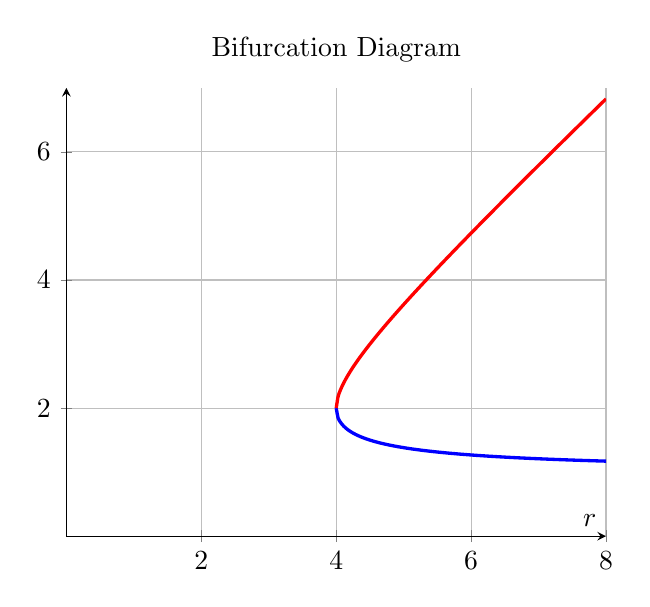
\begin{tikzpicture}
        \begin{axis}[axis lines=center, xlabel={$r$}, title={Bifurcation Diagram}, xmin=0,
            xmax=8, ymin=0, ymax=7, grid]
            \addplot[smooth, very thick, blue, domain=4:8, samples=150] {(1/2)*x-(1/2)*sqrt(x^2-4*x)};
            \addplot[smooth, very thick, red, domain=4:8, samples=150] {(1/2)*x+(1/2)*sqrt(x^2-4*x)};
        \end{axis}
    \end{tikzpicture}
\end{center}
\begin{enumerate}
    \item[(a)] How many equilibrium solutions are there to the differential equation when
        $r<4$? When $r=4$? When $r>4$?
    \item[(b)] Make a plot of $\frac{dy}{dt}$ vs. $y$ assuming that $r > 4$.  Is the blue
        part of the bifurcation diagram stable, unstable or semi-stable?  What about the
        red part?
    \item[(c)] Make a plot of $\frac{dy}{dt}$ vs. $y$ assuming that $r = 4$.  Is the
        single equilibrium point stable, unstable, or semi-stable?
\end{enumerate}
\end{problem}





\newpage\section{Additional Exercises}

\begin{problem}
    Explain how Euler's method works in clear mathematical language.
\end{problem}

\begin{problem}
    It is tempting once you have written computer code for something like Euler's method
    to forget what is actually going on under the hood and just let it act as a {\it black
    box} computational tool.  In this problem you will simply
    take several steps of an Euler solution by hand and graphically so you can mentally
    unpack what Euler's method is doing. Now would be a good time to go back and read the
    section on Euler's Method (Section \ref{sec:Euler}).

    Consider the differential equation $\frac{dy}{dt} = -\frac{ty}{2} + t^2$ with
    initial condition $y(0) = 1$.  We would like to build an Euler approximation on the
    interval $t \in [0,1]$ with a time step of $\Delta t = 0.2$. Use Euler's method to
    give approximations starting at $t=0$ and ending at $t=1$.  Plot your approximate
    solution on the given coordinate plane.  After you've done this by hand use your code
    to get a better approximation using Euler's method with a smaller $\Delta t$.  Compare
    your answers.

    \begin{center}
        \begin{tabular}{|c|c|}
            \hline
            $t$ & Approximation of $y(t)$ \\ \hline \hline
            0 & 1 \\ \hline
            & \\ \hline
            & \\ \hline
            & \\ \hline
            & \\ \hline
            1 & \\ \hline
        \end{tabular}
    \end{center}
    \begin{center}
        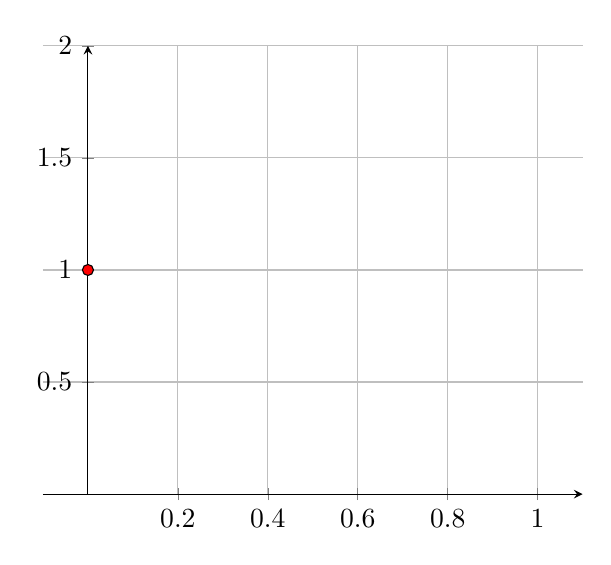
\begin{tikzpicture}
            \begin{axis}[axis lines=center, grid, xmin=-0.1, xmax=1.1, ymin=0, ymax=2]
                \draw[fill=red] (axis cs:0,1) circle(0.07cm);
            \end{axis}
        \end{tikzpicture}
    \end{center}
\end{problem}

\begin{problem}
    Write a differential equation that has four equilibrium points: 2 unstable,
1 stable, and 1 semi-stable.  Support your answer with a plot of
$y'$ vs $y$.

\begin{minipage}{0.5\columnwidth}
    \begin{tikzpicture}
        \draw[<->, thick, black] (-4.5,0) -- (4.5,0) node[anchor=west]{$y$};
        \draw[<->, thick, black] (0,-3) -- (0,3) node[anchor=south]{$dy/dt$};
    \end{tikzpicture}
\end{minipage}
\begin{minipage}{0.5\columnwidth}
    \[ \frac{dy}{dt} = \underline{\hspace{1.5in}} \]
\end{minipage}
\end{problem}
\solution{
    \[ y' = (y-1)(y-2)(y-3)^2(y-4) \]
}

\begin{problem}
    Consider the differential equation $y' = -7(y+3)(y-4)$.  What are the equilibrium
    values of this equation and are they stable, unstable, or semistable? What happens to
    the equilibrium points if
    the $-7$ were changed to $7$ in the differential equation?
\end{problem}
\solution{Hint: Make a plot with $y'$ on the vertical axis and $y$ on the horizontal axis.
}

\begin{problem}
    Newton's Law of Cooling states that the rate of change of the temperature of a cooling
    body (like a coffee in a cup) is proportional to the difference between the current
    temperature and the ambient room temperature.  Write the differential equation
    associated with Newton's Law of Cooling and sketch several solution plots.  Some of
    your plots should be drawn assuming that the initial temperature is greater than the
    ambient temperature and some should be drawn assuming that the initial temperature is
    less than the ambient temperature.
    \begin{center}
        \begin{tikzpicture}
            \begin{axis}[axis lines=center, xlabel={Time}, ylabel={Temp},
                    xtick=\empty, ytick=\empty, xmin=-1.1, ymin=0, ymax=5, xmax=6]
                    \addplot[smooth] {0*x};
                    \draw (axis cs:0.1,3) -- (axis cs:-0.1,3)
                    node[anchor=east]{$T_{amb}$};
                \end{axis}
            \end{tikzpicture}
        \end{center}
\end{problem}
\solution{
    \[ \frac{dT}{dt} = -k(T-T_{amb}) \]
}


\begin{problem}
A skydiver falls out of a plane and free falls toward the ground.
Newton's second law states that the product of the mass and the acceleration
must be equal to the sum of the forces acting on the sky diver.  The two primary forces acting
on the falling sky diver are gravity and air resistance.  A sensor measures the
distance from the plane where it is dropped (positive distance is {\it down} from the
sensor). See the free body diagram below.

\begin{center}
    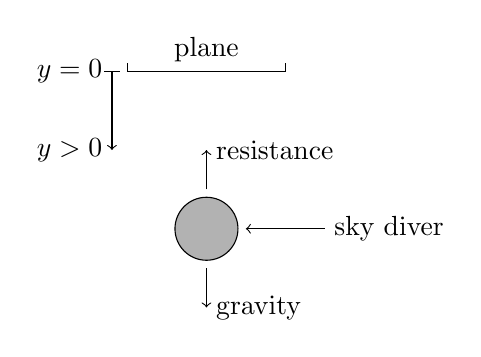
\begin{tikzpicture}
        \draw (-1,0.1) -- (-1,0) -- (1,0) -- (1,0.1);
        \draw (0,0) node[anchor=south]{plane};
        \draw[fill=black!30] (0,-2) circle(0.4cm);
        \draw[<-] (0.5,-2) -- (1.5,-2) node[anchor=west]{sky diver};
        \draw[->] (0,-1.5) -- (0,-1) node[anchor=west]{resistance};
        \draw[->] (0,-2.5) -- (0,-3) node[anchor=west]{gravity};
        \draw (-1.3,0) -- (-1.1,0);
        \draw[->] (-1.2,0) node[anchor=east]{$y=0$} -- (-1.2,-1) node[anchor=east]{$y>0$};
    \end{tikzpicture}
\end{center}

\begin{enumerate}
    \item[(a)] It can be shown experimentally that the air resistance is proportional to the
    square of the velocity.  What differential equation models the \underline{velocity} of
    the falling sky diver? \\(Hints: (1) Recall that if $y(t)$ is the position of the
    falling sky diver then $v(t) = y'(t)$ is the velocity and $a(t) = v'(t) = y''(t)$
    is the acceleration.  \\(2) be sure to get the signs correct!)
    \[ m \cdot \underline{\hspace{0.5in}} = \underline{\hspace{1in}} +
        \underline{\hspace{1in}} \]
        \solution{$mv' = mg - bv^2$}

    \item[(b)] What is the equilibrium solution to the differential equation that you
    proposed in part (a). Discuss the meaning of this equilibrium in the context of the
    problem. Is it stable or unstable? 
    \solution{
        \[ 0 = mg - bv^2 \quad \implies \quad v_{eq} = \sqrt{mg/b} \]
        This is the terminal velocity of the falling sky diver.  This is a stable
        equilibrium.
    }


\item[(c)] Sketch a plot of the velocity and the position functions vs time.  (You do
    not need to solve the differential equation.)
    \begin{center}
        \begin{tikzpicture}[scale=1]
            \begin{axis}[axis lines=center, grid, xmin=0, xmax=2, ymin=0, ymax=4,
                title={Velocity vs. Time}, xlabel={$t$}, ylabel={$v(t)$}, xtick=\empty,
            ytick=\empty]
                \addplot[smooth, black, domain=0:2] {0*x};
%                 \ipa{\addplot[smooth, very thick, red, domain=0:2] {1.96- 1.96*exp(-5*x)};}
            \end{axis}
        \end{tikzpicture}\hspace{0.2in}
        \begin{tikzpicture}[scale=1]
            \begin{axis}[axis lines=center, grid, xmin=0, xmax=2, ymin=0, ymax=4,
                title={Position vs. Time}, xlabel={$t$}, ylabel={$y(t)$}, xtick=\empty,
            ytick=\empty]
                \addplot[smooth, black, domain=0:2] {0*x};
            \end{axis}
        \end{tikzpicture}
    \end{center}


\end{enumerate}
\end{problem}



\begin{problem}[The Combustion Problem]
    Let $T$ be the temperature of a combustible material (e.g. oily rags, dry hay, etc.).
    The conservation of energy equation states that 
    \[ \rho c_p \frac{dT}{dt} = A_1 e^{-B/(T-T_0)} - h\left( T - T_a \right) \]
    where 
    \begin{itemize}
        \item $T$ is temperature in Kelvin,
        \item $T_0$ is a reference temperature above which the fuel starts oxidizing,
        \item $T_a$ is the ambient temperature of the surrounding air,
        \item $\rho$ is the density of the fuel,
        \item $c_p$ is the specific heat of the fuel source, 
        \item $h$ is a measure of the power per volume per degree Kelvin,
        \item $A_1$ is a measure of the power per unit volume, and
        \item $B$ is a rate constant measured in degrees Kelvin.
    \end{itemize}
    If we divide both sides of the differential equation by $\rho c_p$ we arrive at the
    first order non-homogeneous differential equation
    \[ \frac{dT}{dt} = A e^{-B/(T-T_0)} - C \left( T - T_a \right). \]  
    Assume that $A, B,$ and $C$ are all positive coefficients.
    \\{\bf Your Tasks:}
    \begin{enumerate}
        \item[(a)] Why must $T > T_0$ in order for the equation to make sense physically?
        \item[(b)] Let's suppose that $T_a = 300^\circ K$ and that $T_0$ is also at the
            ambient temperature.  Let $A = 20$, $B = 600$, and $C = 0.01$.  Analyze the
            differential equation graphically plotting the phase portrait, identifying
            equilibrium points, and discussing stability of each point.
        \item[(c)] Discuss the physical interpretation of each equilibrium point.
        \item[(d)] Use a numerical solver to get a graphical solution to the differential
            equation under the conditions listed in part (b).
        \item[(e)] Suppose we don't know what $A$, $B$, and $C$ are, but we do know from
            experiments that the three fixed points are $T_1 = T_a = 300^\circ K$, $T_2 =
            670^\circ K$, and $T_3 = 1200^\circ K$.  What can you say about the
            coefficients $A$, $B$, and $C$?
    \end{enumerate}
\end{problem}
\solution{
    \begin{center}
        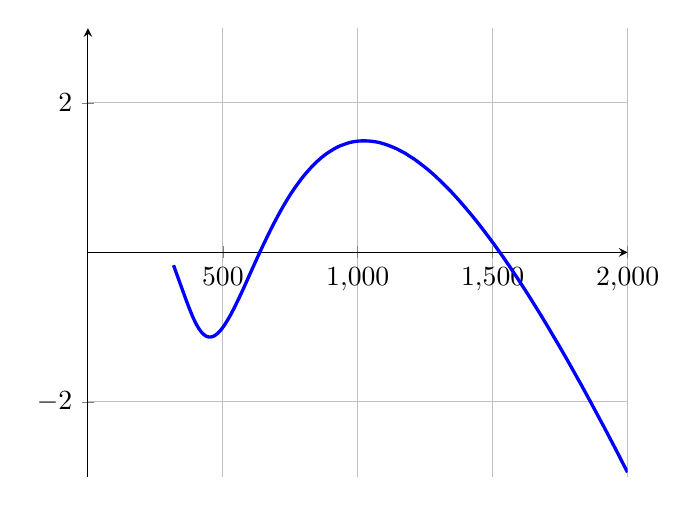
\begin{tikzpicture}
            \begin{axis}[axis lines=center, grid, xmin=0, xmax=2000, ymin=-3, ymax=3,
                domain=300:2000]
                \addplot[smooth, very thick, blue, samples=100] {20*exp(-600/(x-300)) - 0.01*(x-300)};
            \end{axis}
        \end{tikzpicture}
    \end{center}
    The fixed points are $T_1 = 300^\circ K$, $T_2 \approx 636.8^\circ K$, and $T_3
    \approx 1526^\circ K$.  $T_1$ is stable from the right, $T_2$ is unstable (above which
    a combustion occurs), and $T_3$ is stable (stable combustion).
}



